\documentclass[addpoints,12pt]{exam}
\usepackage[lmargin=1.0in,rmargin=1.0in,tmargin=0.75in,bmargin=0.75in]{geometry} 
\usepackage{amsmath, graphicx, float, multicol, enumitem}

% Chemistry Packages
\usepackage[version=3]{mhchem} % Chemistry Formulas
\usepackage{chemfig} % Structures
\usepackage{graphicx}

\setlength{\parindent}{0in}  % No indent on line returns 

\usepackage[T1]{fontenc}
\usepackage{mathpazo} %% Option 'black' gives heavier bold face 
\usepackage{pictex}

% My shortcut section 
\newcommand{\h}{\ce{[H3O^+]} }
\newcommand{\oh}{\ce{[OH^-]} }

\pagestyle{plain}
\pointpoints{pt}{pts}
\bonuspointpoints{pt: bonus}{pts: bonus}

\pagestyle{plain}
\begin{document}
\thispagestyle{empty}
\pagestyle{empty}

{\large\bfseries Chemistry \hfill Chapter 12-13 Review}

\vspace{16pt}
{\bfseries Name: \underline{\hspace{3in}}}

\bigskip

\vspace{0.25in}
\begin{questions}
	\question[1] Label the Acid and Base reactants in the following equation and draw a line to each conjugate:
    \par
    \begin{center}
    \ce{HCO3^-_{(aq)} + H2O_{(l)} <=> H2CO3_{(aq)} + OH^-_{(aq)}}
	\end{center}
\vspace{0.75in}

	\question[1] Find the \oh and pH of a 0.100 M \ce{LiOH} solution.
\vspace{1.5in}

	\question[1] What is the \oh and pH of a 0.225 M \ce{Sr(OH)2} solution?
\vspace{1.5in}

	\question[1] Find the \oh and pH of a 0.010 M \ce{Ba(OH)2} solution.
\vspace{1.5in}

	\question[1] Label the Br\o nsted-Lowry base and its conjugate acid in the following reaction:
    	\begin{center}
    		\ce{NH3_{(aq)} + H2O_{(l)} <=> NH4^+_{(aq)} + OH^-_{(aq)}}
    	\end{center}
\vspace{1.5in}

	\question[1] Draw the movement of electrons in the following Structural Equation and label the Lewis acid and Lewis base.
      \begin{center}
      \small
      \schemestart
              \chemfig{Al
                (-[2]\lewis{0:2:4:,Cl})
                (-[4]\lewis{2:4:6:,Cl})
                (-[6]\lewis{4:6:0:,Cl})
                }
              \+
              \chemfig{\lewis{4:,N}
                   (-[2]H)
                   (-[6]H)
                   (-[0]H)
              }
              \arrow{->}
              \chemfig{Al
                (-[2]\lewis{0:2:4:,Cl})
                (-[4]\lewis{2:4:6:,Cl})
                (-[6]\lewis{4:6:0:,Cl})
                -N
                (-[2]H)
                (-[0]H)
                (-[6]H)
              }
      \schemestop
      \end{center}
\vspace{0.75in}

	\question[4]Identify each substance as an acid or a base and write a chemical equation showing how it is an acid or a base according to the Arrhenius definition.
    	\begin{parts}
    	\part \ce{HNO3_{(aq)}}
        \part \ce{NH4^+_{(aq)}}
        \part \ce{KOH_{(aq)}}
        \part \ce{HC2H3O2_{(aq)}}
    	\end{parts}
\vspace{0.5in}
	\question[4] Write the formula for the conjugate base of each acid.
    	\begin{parts}
    		\part \ce{HCl}
            \part \ce{H2SO3}
            \part \ce{HCHO2}
            \part \ce{HF}
    	\end{parts}
\vspace{1.0in}
	\question[1] These three diagrams represent three different solutions of the binary acid \ce{HA}.  Water molecules have been omitted for clarity and hydronium ions \ce{(H3O^+)} are represented by hydrogen ions \ce{(H^+)}.  Rank the acids in order of decreasing acid strength.
    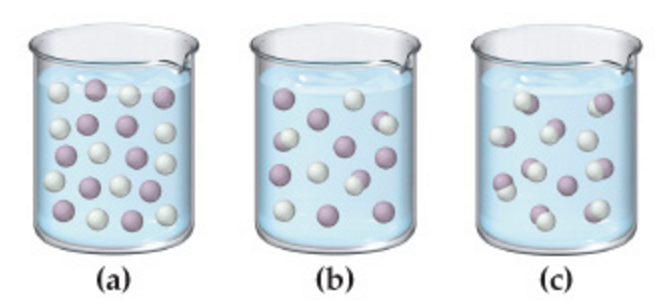
\includegraphics[width=10cm]{3solns.png}
	
    \question[1] Calculate \oh in a solution where the $\h =9.7\times 10^{-9} \text{ M}$.
    \vspace{1.5in}
    
    \question[1] Calculate the pH and pOH of a solution where $\h =2.2\times 10^{-6} \text{ M}$.
\vspace{1.5in}
    \question[3] Calculate the \h and \oh for each solution.
    	\begin{parts}
    		\part pH = 8.55
            \part pH = 11.23
            \part pOH = 11.13
    	\end{parts}
        \vspace{3in}
    \question[1] What mass of \ce{HI} should be present in 0.250 L of solution to obtain a solution with pH = 1.25?
    \vspace{1.5in}
    \question[2] Determine the \h and pH of a 0.200 M solution of Lithium Hydroxide (Assume you have 1.00 L of solution).
    \vspace{1.5in}
    \question[1] Identify the Lewis acid and Lewis base from among the reactants in the following equation:
    \begin{center}
    \ce{Zn^2+_{(aq)} + 4NH3_{(aq)} <=> Zn(NH3)4^2+_{(aq)}}
    \end{center}
    \vspace{1.0in}
    \question[1] Identify the Lewis acid and Lewis base from among the reactants in the following reaction:
    \begin{center}
    \ce{F^-_{(aq)} + BF3_{(aq)} <=> BF4^-_{(aq)}}
    \end{center}
    \vspace{1.0in}
    \question[1] Determine the pH of 0.045 M \ce{Sr(OH)2}.
    \vspace{1.5in}
    \question[1]Write the molecular equation that takes place when aqueous solutions of ammonium chloride and sodium hydroxide are mixed and label the Br\o nsted-Lowry acid and base.
    \vspace{1.5in}
    \question[1] Lactic acid is a weak acid found in milk.  Its calcium salt is a source of calcium for growing animals.  A saturated solution of this salt, which we can represent as \ce{Ca(Lact)2} has a \ce{[Ca^2+]} = 0.26 M.  Assuming the salt is completely dissociated (pretend its actually a strong acid), find its pH.
    \vspace{1.5in}
    \question[1] A solution of 0.23 mol of the chloride salt of protonated quinine \ce{(QH^+)}, a weak organic base, in 1.0 L of solution has pH = 4.58.  Find the concentration of quinine.
    \vspace{1.5in}
    \question[1] Draw the movement of electrons in the following Structural Equation and label the Lewis acid and Lewis base.
      \begin{center}
      \small
      \schemestart
              \chemfig{B
                (-[2]\lewis{0:2:4:,Cl})
                (-[4]\lewis{2:4:6:,Cl})
                (-[6]\lewis{4:6:0:,Cl})
                }
              \+
              \chemfig{H_3C
              -[7]CH_2
              -[1]\lewis{2:6:,O}
              -[7]CH_2
              -[1]CH_3
              }
              \arrow{->}
              \chemfig{
                H_3C
              -[7]CH_2
              -[1]\lewis{6:,O}(-[2,0.75]B(-[2]\lewis{0:2:4:,Cl})(-[4]\lewis{6:2:4:,Cl})(-[0]\lewis{0:2:6:,Cl}))
              -[7]CH_2
              -[1]CH_3
              }
      \schemestop
      \end{center}
\vspace{1.5in}
\end{questions}
\end{document}